%!TEX program = xelatex
%%%%%%%%%%%%%%%%%%%%%%%这是导言部分的开始%%%%%%%%

%========= 导言部分声明文档的类型=================
\documentclass{article}

	%=========导言部分可可以加载宏包=================
	\usepackage{amsmath}                % 数学公式排版宏包
	\usepackage{amssymb}                % 数学符号命令宏包
	\usepackage{amsthm}                 % 数学定理宏包
	\usepackage[UTF8]{ctex}             % 中文输入宏包
	\usepackage[a4paper]{geometry}      % 页面设置宏包
	\usepackage{setspace}               % 行间距宏包
	\usepackage{graphicx}               % 图片宏包
	\usepackage{listings}               % 代码宏包
	\usepackage{color}					% 颜色宏包
	\usepackage{xcolor}                 % 颜色处理宏包
	\usepackage{float}                  % 浮动对象式样宏包
	\usepackage{fontspec}
	\usepackage{enumerate}				% 列举编号包
	
	%=========页面设置==============================
	\geometry{left=1cm,right=1cm,top=1cm,bottom=2cm}
	\onehalfspacing
	\setlength\parindent{0em}

	%=========代码格式设置============================
	\definecolor{dkgreen}{rgb}{0,0.6,0}
	\definecolor{gray}{rgb}{0.5,0.5,0.5}
	\definecolor{mauve}{rgb}{0.58,0,0.82}
	% \setmonofont{Consolas}
	\lstset{
		numbers = left, 	
		numberstyle = \color{gray}, 
		keywordstyle = \color{blue},
		commentstyle = \color{dkgreen}, 
		stringstyle = \color{mauve},
		basicstyle = \ttfamily,
		breaklines = true,
		frame = shadowbox, % 阴影效果
		rulesepcolor = \color{ red!20!green!20!blue!20} ,
		escapeinside = ``, % 英文分号中可写入中文
		xleftmargin = 2em,xrightmargin=2em, aboveskip=1em,
		framexleftmargin = 2em
	} 

%=========导言部分可以定义标题信息===============
\title{组会报告}
\author{徐益}
\date{\today}

%%%%%%%%%%%%%%%%%%%%%%%这是导言部分的结束%%%%%%%%%

%%%%%%%%%%%%%%%%%%%%%%%这是正文部分的开始%%%%%%%%%
\begin{document}

%=========生成标题================================
\maketitle

%=========开始正文的输入==========================

%===========第一节=================
\section{工作内容}

1. 完成5GNR中LDPC相关的matlab仿真

2. 用C语言实现5GNR中的LDPC编译码

%===========第一节=================
\section{5GNR中LDPC相关的matlab仿真}

\subsection{误码性能仿真}
\begin{figure}[H]
	\centering
	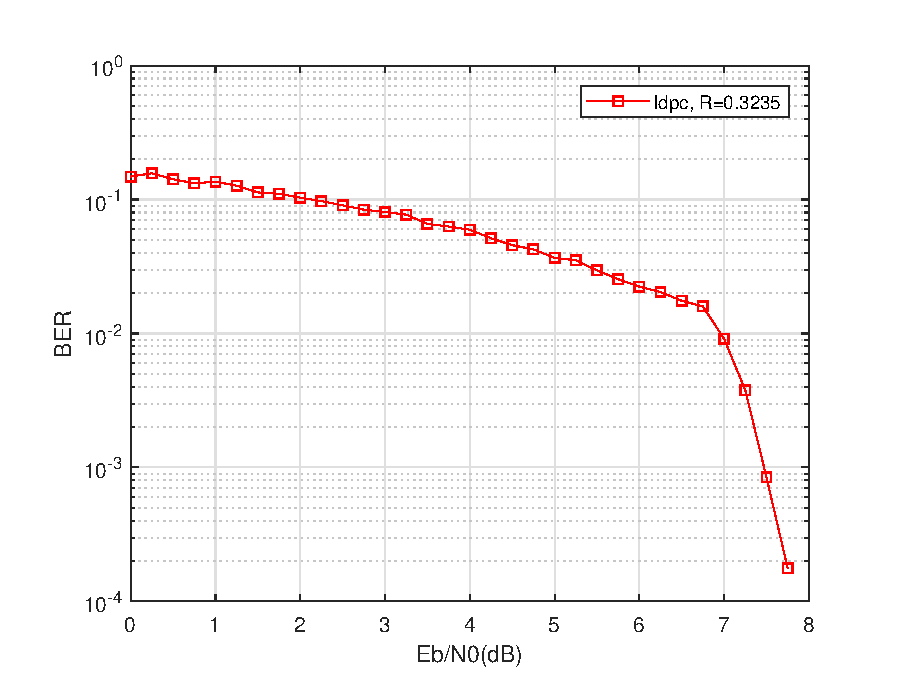
\includegraphics[width = .8\textwidth]{error.eps}
	\caption{基于min-sum算法的LDPC译码误码性能(错误)}
\end{figure}
问题:文献\emph{A Bit-Serial Approximate Min-Sum LDPC Decoder and FPGA Implementation}
中min-sum算法介绍的变量节点信息更新公式(式(2))缺一项。

\begin{figure}[H]
	\centering
	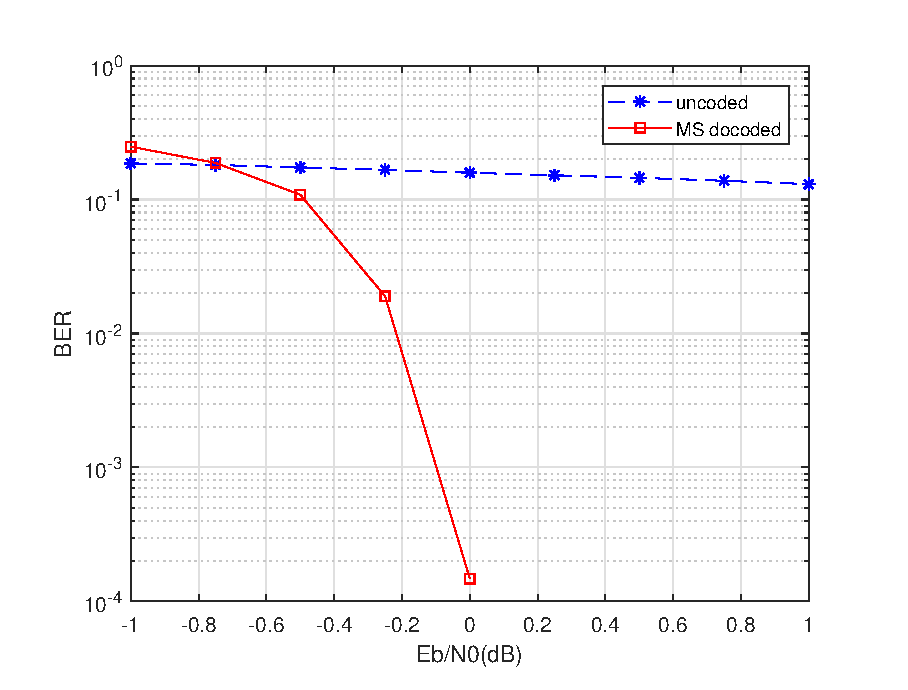
\includegraphics[width = .8\textwidth]{ms.eps}
	\caption{基于min-sum算法的LDPC译码误码性能(R=11/34)}
\end{figure}

\begin{figure}[H]
	\centering
	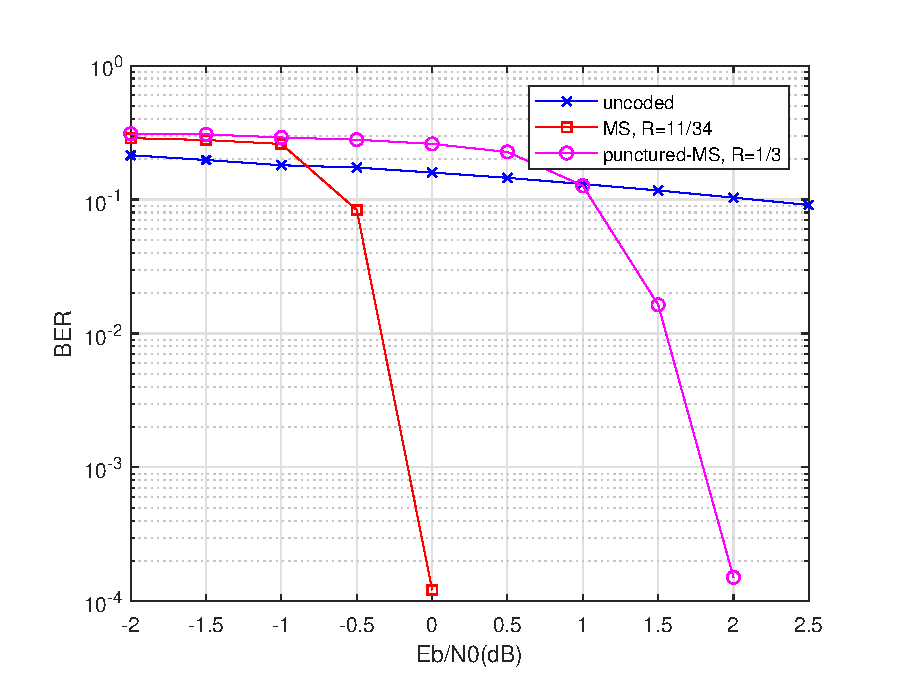
\includegraphics[width = .8\textwidth]{pun.eps}
	\caption{基于打孔的min-sum算法的LDPC译码误码性能}
\end{figure}

\subsection{其余部分仿真}
\begin{figure}[H]
	\centering
	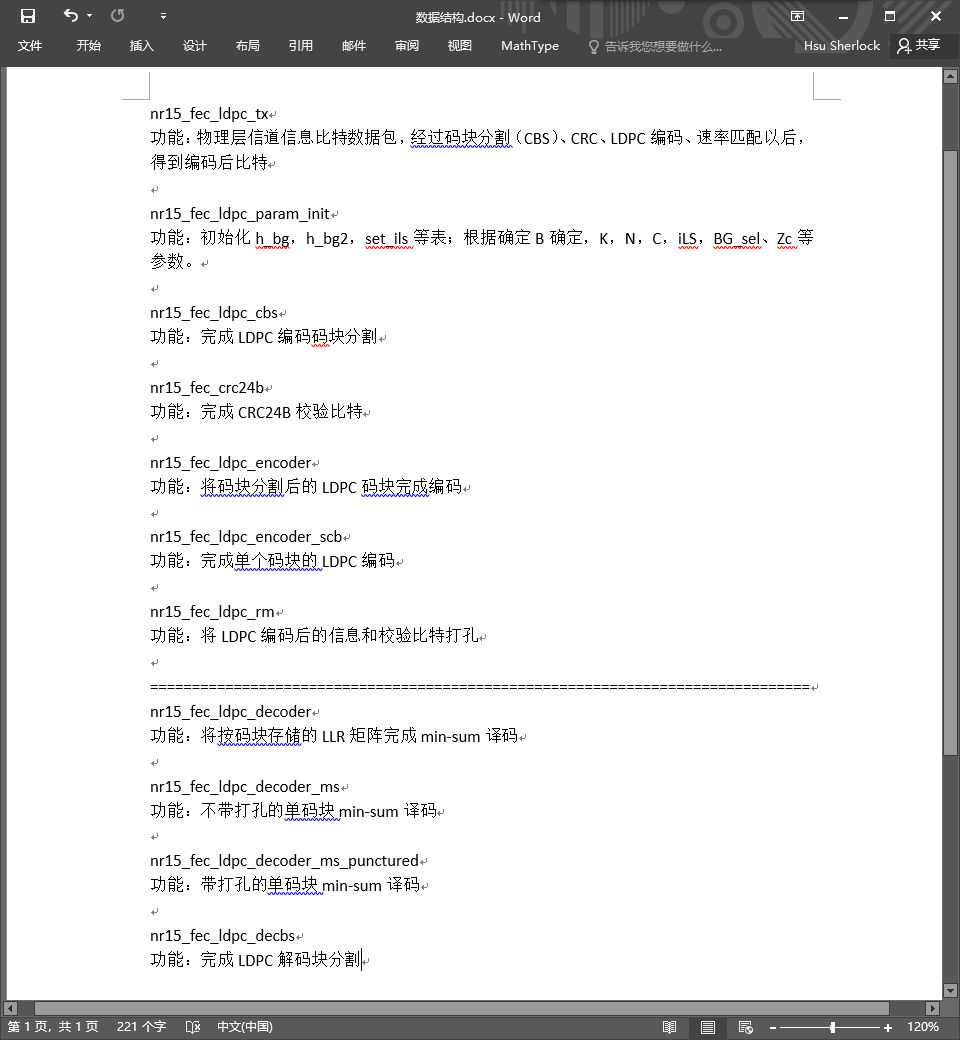
\includegraphics[width = .8\textwidth]{document.png}
	\caption{matlab代码说明文档}
\end{figure}

%===========第二节=================
\section{用C语言实现5GNR中的LDPC编译码}


%===========第三节=================
% \section{修改流量控制方式}


%===========第四节=================
% \section{其他改进方向}
% 1. 选择更大的DPDK发送页。\\

% 2. 选择更优的流量控制策略。\\

%===========下周计划=================
\section{下阶段计划}
1. 继续用C语言实现5GNR中的LDPC编译码

\end{document}
%%%%%%%%%%%%%%%%%%%%%%%这是正文部分的结束%%%%%%%%%%%%